\subsection{Seven segment decoder}

\begin{figure}[htbp]
   \centering
   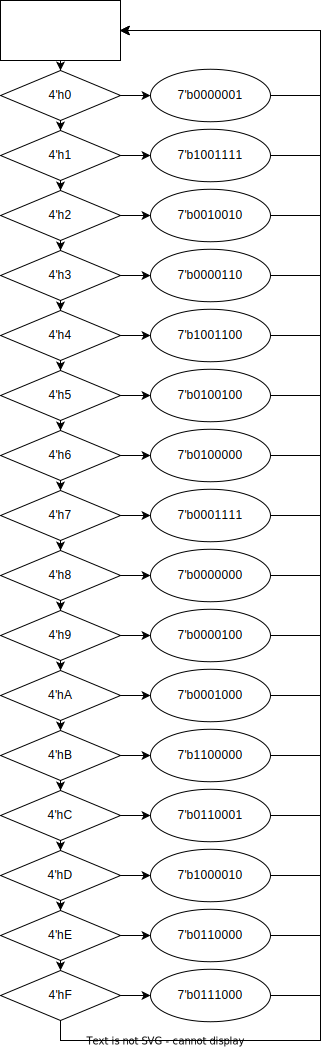
\includegraphics[width=0.85\textwidth]{seven_segment_decoder_asm.png}
   \caption{ASM chart of seven segment decoder module.}
   \label{fig:seven_segment_decoder_asm}
\end{figure}

\begin{minted}[
   fontsize=\footnotesize,
   linenos,
   breaklines,
]{verilog}
// decoder: convert coded input into conded output
/**
For Altera DE2,

  -a-
f|   |b
  -g-
e|   |c
  -d-

displays 0123456789ABCDEF
*/
module seven_seg_dec (
	input [3:0] bcd_i,  // binary coded decimal input
	output reg [6:0] out_o
);

always @(bcd_i)
	case (bcd_i)
		//               abcdefg
		4'h0: out_o = 7'b0000001;
		4'h1: out_o = 7'b1001111;
		4'h2: out_o = 7'b0010010;
		4'h3: out_o = 7'b0000110;
		4'h4: out_o = 7'b1001100;
		4'h5: out_o = 7'b0100100;
		4'h6: out_o = 7'b0100000;
		4'h7: out_o = 7'b0001111;
		4'h8: out_o = 7'b0000000;
		4'h9: out_o = 7'b0000100;
		default: out_o = 7'b1111111;
	endcase

endmodule
\end{minted}
